\chapter{Einleitung}

\section{Motivation und Problemstellung}

Feedback Bernd: Wenn die Kunden auf den Preis schauen, muss der Anbieter nicht zwingend Kosten reduzieren, kann aber auch die Leistung erhöhen, um den Preis zu rechtfertigen; 2022 29\% wie war es denn vorher; Quellen fehlen; Kunde und Kontakt zu häufig; Wettbewerbsfähig zu sein und zu bleiben 

Die digitale Transformation verändert sowohl das private als auch das geschäftliche Umfeld grundlegend. Das stellt auch die eher träge auf Veränderungen reagierende deutsche Versicherungsbranche vor neue Herausforderungen. So erleichtert die Digitalisierung Kunden den Zugang zu Informationen, beschleunigt Versicherungsabschlussprozesse und ermöglicht das Vergleichen von Anbietern. Besonders deutlich zeichnen sich diese Veränderungen in der Kfz-Versicherungsbranche ab. So hat eine Studie von Statista aus dem Jahr 2022 ergeben, dass die Kfz-Versicherungssparte mit mehr als 25 \% online abgeschlossener Verträge in Deutschlandland in der Versicherungsbranche aktuell führend ist.

Bei der Wahl des Anbieters ist dabei für die Kunden der Preis der ausschlaggebende Faktor, weshalb Kfz-Versicherer ihre Kosten reduzieren müssen, um für neue Kunden attraktiv zu bleiben. Diese Vergleichbarkeit bei sehr ähnlichen Produkten führt ebenfalls dazu, dass in Deutschland 2022 29 \% der Versicherungsnehmer ihren Kfz-Versicherungsanbieter wechselten. Eine Ursache hierfür ist der mangelnde Kundenkontakt und die daraus resultierende niedrige Kundenloyalität. Kfz-Versicherer haben hier das Problem, dass sie mit dem Kunden in der Regel nur beim Vertragsabschluss und im Schadenfall Kontakt haben. Daher ist es laut dem Vertriebsvorstand der Neodigital Versicherung AG Stephen Voss umso wichtiger, dass die wenigen Kontaktpunkte einfach, schnell und praktisch ablaufen, sodass der Versicherungsanbieter von Kunden nicht negativ wahrgenommen wird. 

Folglich müssen Kfz-Versicherer ihre internen Prozesse zur Kostenreduktion optimieren und ihren digitalen Auftritt verbessern, um  langfristig am Markt wettbewerbsfähig zu sein bzw. zu bleiben. Für diese digitale Transformation ist nicht eine einzelne Komponente entscheidend, sondern benötigen die Kfz-Versicherer vielmehr eine digitale Plattform, mit der interne Prozesse digitalisiert, Anwendungen integriert und zudem das Anbieten von weiteren Services für den Endkunden ermöglicht wird.

%\newpage
\section{Zielsetzung und Abgrenzung}

Die SAP Business Technology Plattform ist eine digitale Plattform, mit der Kfz-Versicherer ihre bestehende IT-Landschaft transformieren und an neue Geschäftsanforderungen anpassen können.

Ziel dieser Arbeit ist es daher, die Anforderungen der Kfz-Versicherer an eine digitale Plattform zu identifizieren, um anschließend beurteilen zu können, inwiefern die Anforderungen der Kfz-Versicherer an eine digitale Plattform von der SAP Business Technology Plattform erfüllt werden. Die aus der Analyse resultierende Handlungsempfehlung soll Kfz-Versicherern eine praxisorientierte Vorgehensweise zur Implementierung der SAP Business Technology Plattform aufzeigen.

\improvement{Muss ich hier aus dem Inwiefern nicht nochmal ein ob machen?}
Dabei wird der deutsche Kfz-Versicherungsmarkt betrachtet, da eine Analyse inklusive internationaler Märkte aufgrund der unterschiedlichen regulatorischen Rahmenbedingungen, divergierender Prämienfaktoren sowie ungleichmäßig ausgeprägter technologischer Fortschritte nicht hinreichend aussagekräftig wäre. Des Weiteren konzentriert sich die Arbeit im Wesentlichen auf die technologischen Merkmale einer digitalen Plattform. Darüber hinaus werden im Rahmen dieser Untersuchung digitaler Plattformen als Wettbewerbsfaktor betrachtet, nicht aber in Bezug zu anderen Wettbewerbskräften im Versicherungsmarkt gesetzt.



\newpage
\section{Aufbau der Arbeit}

Zu Beginn der Projektarbeit werden zunächst digitale Plattformen als disruptive Innovation erläutert. Hierzu werden digitale Plattformen definiert, die Wertschöpfung digitaler Plattformen vorgestellt, Cloud-Computing auf technischen Plattformen beschrieben und darauf aufbauend die SAP Business Technology Platform vorgestellt. Danach werden die Definition und Grundprinzipien der Versicherung sowie der Aufbau und der Wettbewerb in der Kfz-Versicherungssparte dargestellt. Anschließend wird die Wahl der wissenschaftlichen Methodik begründet und das Vorgehen bei der Task-Technology-Fit-Theorie, der systematischen Literaturanalyse, dem semistrukturierten Leitfadeninterview sowie bei der qualitativen Inhaltsanalyse beschrieben. Danach werden die Anforderungen der Kfz-Versicherer an digitale Plattformen mithilfe der systematischen Literaturanalyse identifiziert und anschließend mittels Experteninterviews ergänzt und evaluiert. Daraufhin werden die Funktionalitäten und Services der SAP \ac{btp} vorgestellt, um diese im Anschluss den Anforderungen der Kfz-Versicherer gegenüberzustellen. Ausgehend von dem Analyseergebnis wird eine Handlungsempfehlung für deutsche Kfz-Versicherer ausgesprochen. Darauffolgend werden die Vorgehensweise und Analyseergebnisse kritisch reflektiert, um abschließend die Arbeit mit einem Fazit zusammenzufassen und in einem Ausblick mögliche Folgeuntersuchungen aufzuzeigen.(siehe Abbildung \ref{fig:Aufbau})


\begin{figure}[h]
    \centering
    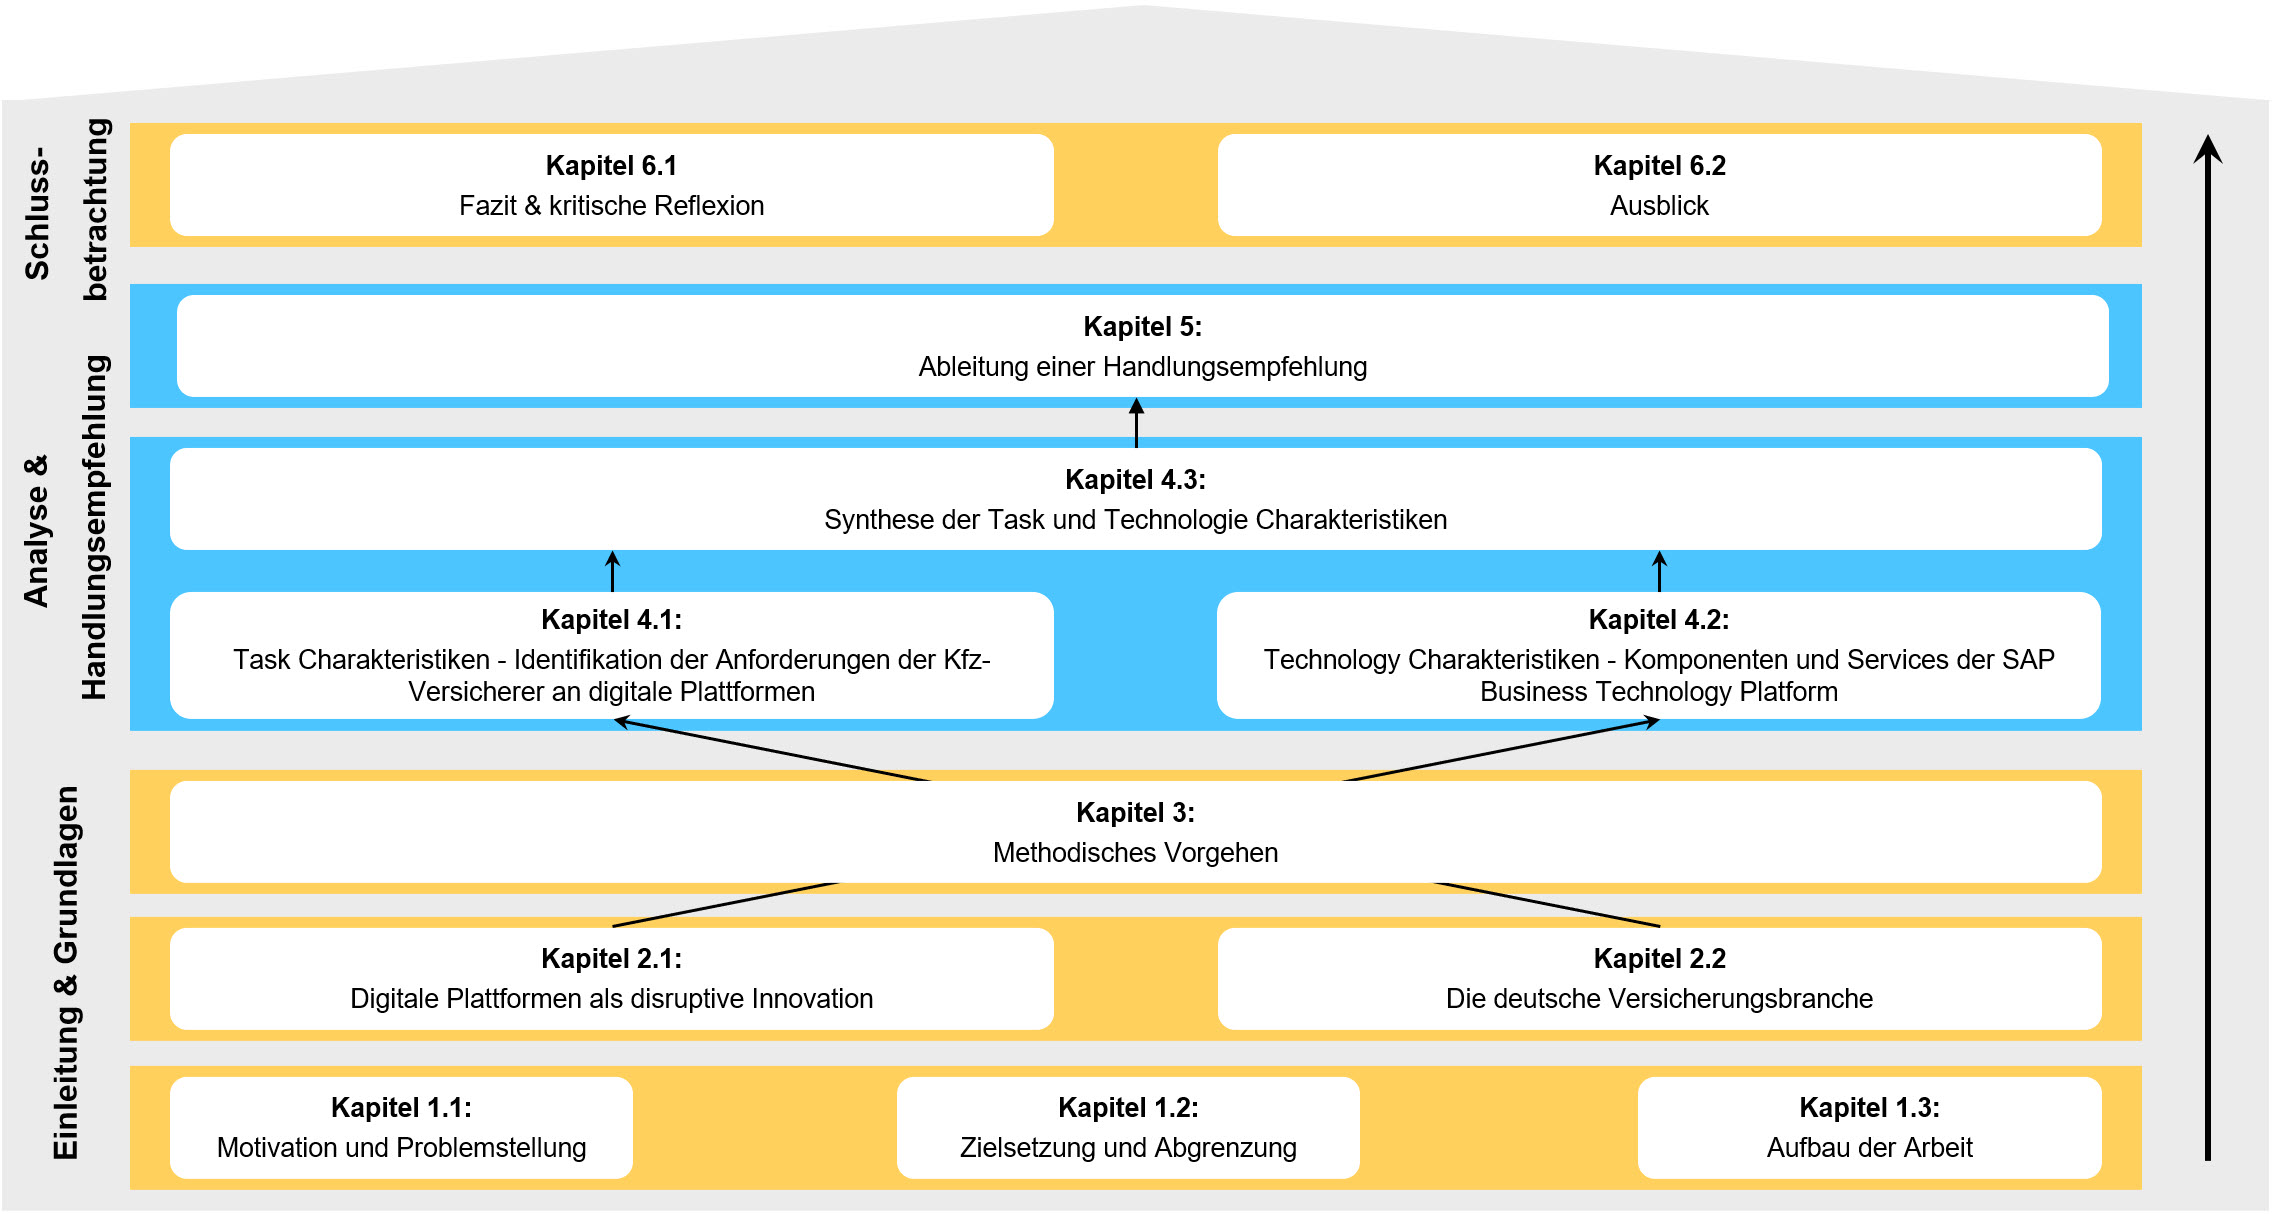
\includegraphics[width=1\textwidth]{img/Aufbau_der_Arbeit.jpg}
    \caption[Aufbau der Arbeit]{Aufbau der Arbeit\autocite{Aufbau}}
    \label{fig:Aufbau}
\end{figure}
\footnotetext{eigene Darstellung}

\improvement{Feedback Bernd: Pfeile nicht überkreuzen und Bild größer}

\newpage